\section*{Problem 3}

The task was to implement the vector rally game -- which basically is
interactive, gamified vector addition.

A key feature of the game is that the walls of the map must not be crossed as
it would be equivalent of crashing the car. A reliable and general method of
detecting intersections between the cars movement vector and the walls is
needed.

The cars movement can be represented as line segment with following parameter
$$ (x, y) = (x_0, y_0) + t (\Delta x, \Delta y) $$
and in a similar fashion a wall segment can be represented as two points with
one as the origin and one as the direction vector
$$ (x, y) = (a_0, b_0) + s (\Delta a, \Delta b) $$
When these expressions are equal, the lines intersect. If the $t$ and $s$
factor are both satisfy $t, s \in [0,1]$ then the lines intersect between
their defining points -- in the game this translates to a collision.

This matrix represents the relationship and the equation

$$
\begin{bmatrix*}[c]
 \Delta x & -\Delta a & a_0 - x_0 & 0 \\
 \Delta y & -\Delta b & b_0 - y_0 & 0\\
\end{bmatrix*}
$$

Solving yields the following equations for calculating the 
intersecting point:

$$ t = \frac{-b_0 \Delta a + y_0 \Delta a + a_0 \Delta b - x_0 \Delta b}{\Delta b \Delta x - \Delta a \Delta y} $$
$$ s = \frac{-b_0 \Delta x + y_0 \Delta x + a_0 \Delta y - x_0 \Delta y}{\Delta b \Delta x - \Delta a \Delta y} $$

These calculations can be used and implemented directlt in Java since they
only contain simple calculations.

There is however a special case: If the two lines are parrallel there is no
need to test for intersections.

The procedure to detect an intersection is to:
\begin{enumerate}
\item Determine whether the lines segments are parallel
\item Caculate their deltas ($\Delta a$, $\Delta b$, $\Delta x$ and $\Delta y$)
\item Calculate $t$ and $s$ using above equations
\item If $t$ and $s$ both satisfy $t, s \in [0,1]$: Then the lines intersect
\end{enumerate}

This method is completely general and applies to any kind of line intersection
-- boundaries, goal lines or items. In the program it is implemented as the
method \code{intersects}.

\subsection*{Boundaries and goal lines}

The general line intersection detection makes it easy to implement boundaries
and goal lines.

When an obstacle is added to the map, the line segments corresponding to the
edges are added to an array. This global array containes each line segment as
a two-cell array containing start and end point. By looping over each element
in the boundary array, intersections can be detected. Since arrays are used
this puts an upper limit on the number of edges to account for (1024 in the
solution.)

The goal line uses the same code to check for intersections but here the
program must also detect if the car is driving in the right direction.
This is done by taking the dot product of a vector orthorgonal to
the goal line and a vector that is the sum of the vector representing
the distance moved last turn and the one representing the distance to move
in the current turn. Depending on the reference direction, the dot product
will either be positive when the goal line is crossed from the right direction
and negative when crossed from the wrong one, or vice versa.

The might sound complicated, but it is neccessary to support goal lines
that are not parallel to either the x-axis or y-axis of the coordinate system.

\subsection*{Wrong way detection}
A crude form of wrong way detection can be implemented by recording
the crossing of goal lines as described in the previous section.
Each time the car crosses the line in the wrong direction, a counter
is simply decremented, and oppositely incremented when the car crosses
in the right direction. If we say the counter is initalized to zero, the player
will be notified of driving in the wrong direction when it is below zero, and
will be notified of his/her victory when it is equal to 1.

\subsection*{Custom maps}
Custom maps can be implemented by having the game read the map data from a file.
A good compromise between human readability (since there will be no map editor)
and machine readability is a plain text file that is easy to parse.
Below is an example of such a file:
\begin{Verbatim}
12 12 25 25
25 25 40 40

25 37 25 50

26 45
\end{Verbatim}
Each of the lines from the top of the file and downto the first empty line
represents a set of coordinates for two corners of a rectangle. This
rectangle is an obstacle, that will cause you to lose the game, if you
crash into it.

The next line with numbers represents a set of coordinates for the start
and end of the goal line.

Finally the last line represent the coordinates for the starting point - i.e.
the point where a player will start with his/her car when having just started
the game.

Due to this simplicity, the file can be parsed by just reading it line by line,
splitting each line in 4, and creating the various geometric elements on the fly.
In case the file doesn't exist, is not given on the command line or is wrongly formatted,
exceptions are thrown, and subsequently handled by logic in the main method
that will print a nice error message to the user.

\subsection*{Testing}
Below is shown a series of test invokations of the game to demonstrate how
it works and how it handles various special conditions.
First how the program behaves, if it is not given a map to load:
\begin{Verbatim}
java VectorRally              
Please start the game like this: java VectorRally <mapfile>
\end{Verbatim}

Then if it is given more than one argument:
\begin{Verbatim}
java VectorRally centerbox.map hardmap.map 
Please start the game like this: java VectorRally <mapfile>
\end{Verbatim}

If it is given a file that doesn't exist:
\begin{Verbatim}
java VectorRally somefile.map             
Error opening somefile.map: File doesn't exist
\end{Verbatim}

If the file is formatted wrongly (too many empty lines):
\begin{Verbatim}
java VectorRally hardmap.map 
Error parsing hardmap.map: Encountered more than 2 blank lines
\end{Verbatim}

Now finally, when the arguments are correct, the program starts up, but if you crash into an obstacle, you can see what happens
by looking at figure \ref{fig:crash}
\begin{figure}[p]
	\centering
	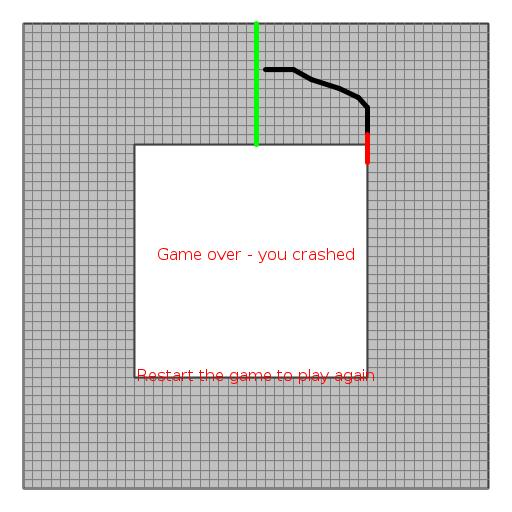
\includegraphics[width=0.8\textwidth]{crash.jpg}
	\caption{Crash}
	\label{fig:crash}
\end{figure}

When one wins, it will look as on figure \ref{fig:win}.
\begin{figure}[p]
	\centering
	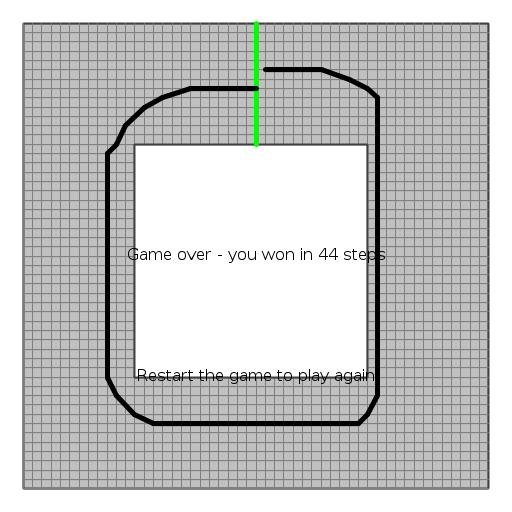
\includegraphics[width=0.8\textwidth]{win.jpg}
	\caption{Winning}
	\label{fig:win}
\end{figure}

And when one drives the wrong way, the player will be warned in the terminal:
\begin{Verbatim}
java VectorRally centerbox.map 
Wrong way!
Wrong way!
Wrong way!
Wrong way!
Wrong way!
Wrong way!
\end{Verbatim}

